\chapter{Otak yang Memerintah}\label{ch:g5:brain-in-command}

Sebuah bola melayang ke arahmu; kamu menangkapnya. Setengah detik,
sama sekali tanpa berpikir --- namun dalam setengah detik itu, matamu
melaporkan sebuah benda yang terbang, sesuatu menghitung lintasannya,
dan berlusin-lusin \omterm{def:g3:bones-and-muscles:muscle}{otot} diperintahkan melakukan tangkapan yang persis
tepat. Sesuatu itu adalah \omterm{def:g5:brain-in-command:system}{otak}, dan bab ini mengikuti perintahnya di
sepanjang kabel tubuh.

\section{Jaringan komando}

\begin{definition}[Sistem saraf]\label{def:g5:brain-in-command:system}
Yang disebut \emph{sistem saraf}\index{sistem saraf} adalah jaringan
komando tubuh:
\begin{itemize}
  \item \emph{otak}\index{otak}, di dalam naungan \omterm{def:g3:bones-and-muscles:skeleton}{tengkorak}
        (\cref{def:g3:bones-and-muscles:skeleton}), adalah pusatnya:
        ia menerima semua laporan dan mengeluarkan semua perintah;
  \item \emph{sumsum tulang belakang}\index{sumsum tulang belakang},
        sebuah kabel tebal jaringan saraf, berjalan dari otak turun ke
        dalam tiang pelindung \omterm{def:g4:classifying-animals:vertebrate}{tulang belakang};
  \item \emph{saraf}\index{saraf}, benang putih yang bercabang dari
        otak dan sumsum \omterm{def:g4:classifying-animals:vertebrate}{tulang belakang} ke setiap organ, membawa
        pesannya --- dengan kecepatan lebih dari
        \qty{100}{m/s} bagi yang tercepat.
\end{itemize}
\end{definition}

\begin{proposition}[Melapor, memutuskan, memerintah]\label{prop:g5:brain-in-command:loop}
Setiap tindakan menjalankan gelang yang sama
(\cref{prop:g1:the-five-senses:brain} adalah sketsa pertamanya):
\begin{enumerate}
  \item \emph{\omterm{def:g1:the-five-senses:sense}{alat indra}} melapor: \omterm{def:g5:brain-in-command:system}{saraf} membawa pesannya \emph{ke}
        \omterm{def:g5:brain-in-command:system}{otak};
  \item \emph{\omterm{def:g5:brain-in-command:system}{otak}} merangkai laporannya, memutuskan, lalu menyusun
        perintah;
  \item \omterm{def:g5:brain-in-command:system}{saraf} membawa perintahnya \emph{dari} \omterm{def:g5:brain-in-command:system}{otak} ke
        \emph{\omterm{def:g3:bones-and-muscles:muscle}{otot}} (\cref{def:g3:bones-and-muscles:muscle}), yang
        \omterm{def:g3:bones-and-muscles:muscle}{berkontraksi} atas perintah.
\end{enumerate}
\omterm{def:g1:the-five-senses:sense}{Alat indra} melapor, \omterm{def:g3:bones-and-muscles:muscle}{otot} menurut --- tidak satu pun pernah memutuskan.
\end{proposition}
\admitted

\begin{omfigure}
\begin{tikzpicture}
  % eye
  \draw[thick] (-0.7,1.7) ellipse (0.5 and 0.28);
  \fill[omDef] (-0.58,1.7) circle (0.13);
  \node[font=\small, align=center] (eye) at (-0.7,0.85)
    {mata melihat\\ bolanya};
  % brain
  \draw[thick, omDef, fill=omDef!8, rounded corners=8pt]
    (3.2,1.15) rectangle (6.4,2.45);
  \node[font=\small\bfseries, omDef] at (4.8,2.05) {otaknya};
  \node[font=\footnotesize] at (4.8,1.55) {memutuskan tangkapannya};
  % muscle
  \draw[thick, omThm, fill=omThm!15]
    (9.6,1.5) .. controls (10.0,1.85) and (10.6,1.85) .. (11.0,1.55)
    .. controls (10.6,1.35) and (10.0,1.35) .. (9.6,1.5);
  \node[font=\small, align=center] at (10.3,0.85)
    {otot lengannya\\ berkontraksi};
  % arrows
  \draw[->, very thick, omMeth] (-0.1,1.7) -- (3.1,1.8)
    node[pos=0.42, above=2pt, font=\footnotesize, omMeth]
    {laporan, menyusuri saraf};
  \draw[->, very thick, omProp] (6.5,1.8) -- (9.5,1.6)
    node[pos=0.5, above=2pt, font=\footnotesize, omProp]
    {perintah, menyusuri saraf};
\end{tikzpicture}

{\small Gelang setiap tindakan: laporan kepada \omterm{def:g5:brain-in-command:system}{otak}, keputusan,
perintah kepada \omterm{def:g3:bones-and-muscles:muscle}{otot}.}
\end{omfigure}

\begin{example}[Tangkapan itu, diputar ulang pelan-pelan]\label{ex:g5:brain-in-command:catch}
Putar ulang setengah detiknya: \omterm{def:g1:the-five-senses:sense}{mata} mengikuti bolanya lalu melapor,
terus-menerus; \omterm{def:g5:brain-in-command:system}{otaknya}, dengan membandingkan laporan demi laporan,
menghitung di mana bolanya akan berada; perintah mengalir keluar ke
\omterm{def:g1:my-body:parts}{tungkai} (satu langkah ke kiri), batang tubuh (condong), \omterm{def:g1:my-body:parts}{lengan} dan
jari (buka --- sekarang tutup). Tidak ada satu organ pun yang
``menangkap bolanya'': \omterm{def:g1:the-five-senses:sense}{mata}, \omterm{def:g5:brain-in-command:system}{otak} dan \omterm{def:g3:bones-and-muscles:muscle}{otot} masing-masing memainkan
barisnya pada \cref{prop:g5:brain-in-command:loop}.
\end{example}

\begin{remark}[Lebih daripada gerakan]\label{rem:g5:brain-in-command:more}
\omterm{def:g5:brain-in-command:system}{Otak} yang sama yang menangkap bola juga menyimpan ingatanmu, menahan
perhatianmu pada halaman ini, bermimpi pada malam hari --- dan
menjalankan layanan yang tidak pernah kamu pikirkan: ia menjaga
\omterm{def:g4:breathing:movements}{pernapasan} tetap berjalan siang dan malam
(\cref{def:g4:breathing:movements}) dan menyetel irama \omterm{def:g4:heart-and-blood:heart}{jantung}
terhadap kebutuhan tubuh
(\cref{ex:g4:heart-and-blood:effort}). Sebagian perintah adalah
milikmu untuk diberikan; sebagian lagi diberikan \omterm{def:g5:brain-in-command:system}{otak} untukmu.
\end{remark}

\section{Mengukur gelangnya: waktu reaksi}

\begin{definition}[Waktu reaksi]\label{def:g5:brain-in-command:reaction}
Gelangnya cepat tetapi tidak seketika: laporan, keputusan dan perintah
masing-masing mengambil bagiannya. Jeda antara sebuah isyarat dan
tanggapan tubuh disebut \emph{waktu reaksi}\index{waktu
reaksi} --- untuk tugas sederhana (menangkap, menekan, meraih),
kira-kira seperlima detik pada orang yang terlatih, sedikit lebih lama
pada anak-anak.
\end{definition}

\begin{method}[Uji penggaris]\label{met:g5:brain-in-command:ruler}
\omterm{def:g5:brain-in-command:reaction}{Waktu reaksi} tanpa alat apa pun kecuali sebuah penggaris:
\begin{enumerate}
  \item seorang teman memegang sebuah penggaris yang menggantung
        tegak, tanda nol di bawah, di antara ibu jari dan jarimu yang
        terbuka;
  \item tanpa aba-aba, temannya melepaskannya; kamu menangkap
        penggarisnya secepat mungkin;
  \item bacalah di mana kamu menangkapnya: makin sedikit sentimeter
        yang meluncur lewat, makin cepat gelangmu;
  \item ulangi beberapa kali lalu simpan nilaimu yang lazim --- sekali
        percobaan melompat ke sana ke mari.
\end{enumerate}
Penggaris yang jatuh mengubah waktu menjadi sentimeter: kira-kira
$\qty{15}{cm}$ berpadanan dengan seperenam detik.
\end{method}

\begin{omfigure}
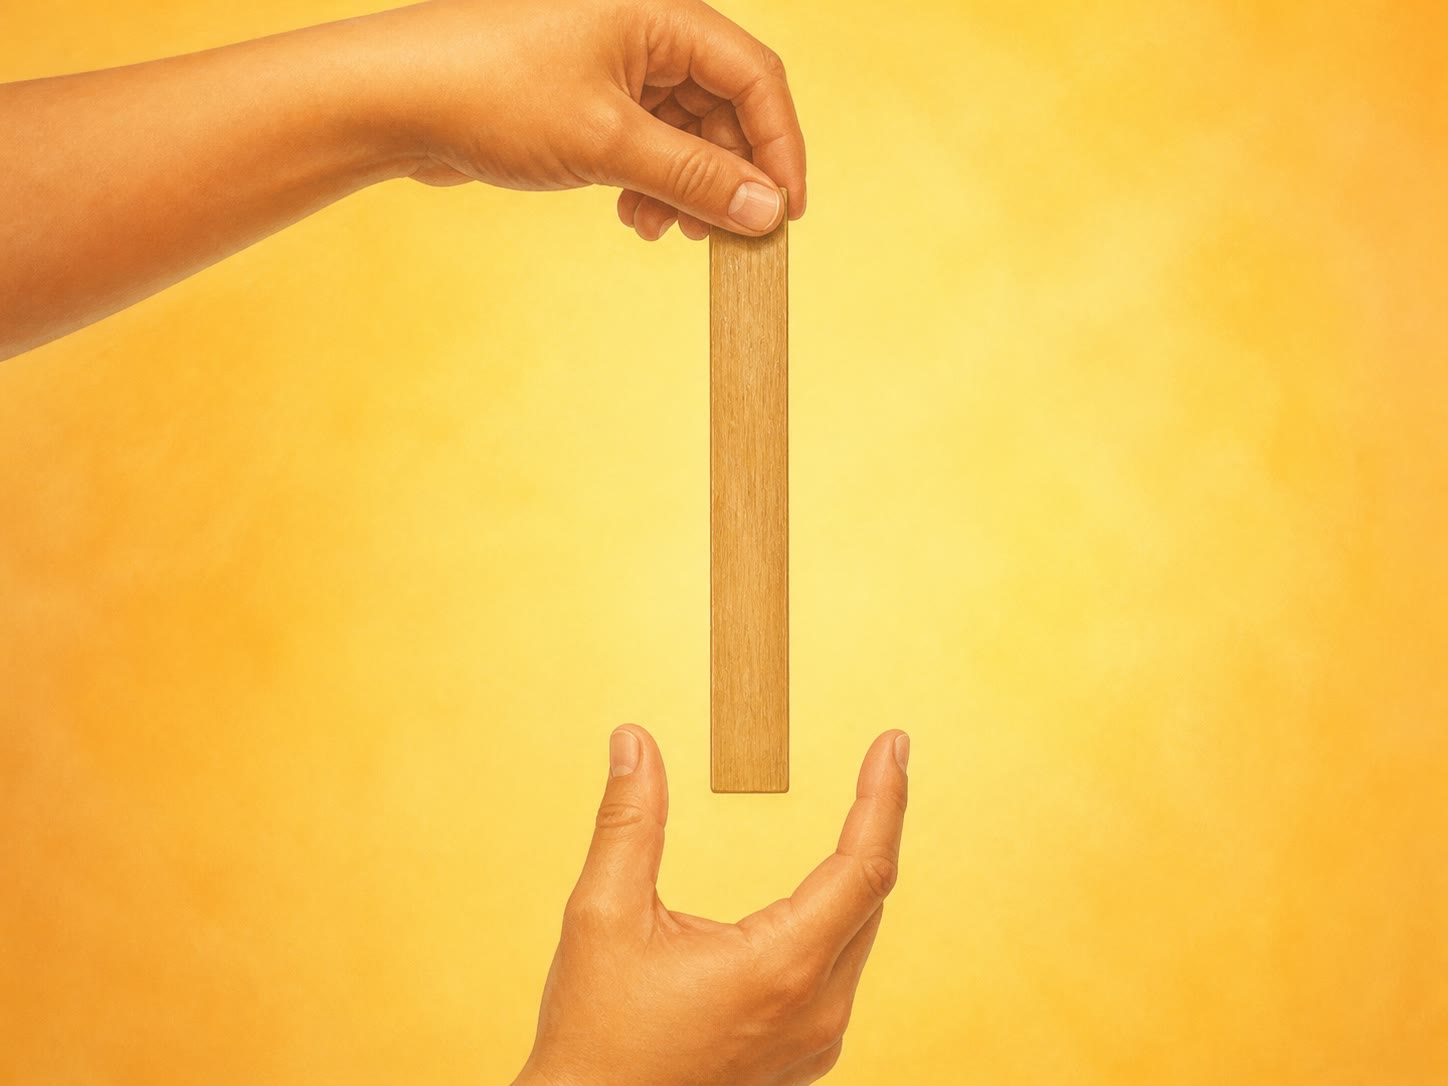
\includegraphics[width=0.5\linewidth]{images/book1/ai/g5-brain-ruler.jpg}

{\small Uji penggarisnya, sekejap sebelum jatuhnya: ketika tangan yang
di atas melepaskannya, gelang tangan yang di bawah --- melihat,
memutuskan, menutup --- memulai seperlima detiknya.}
\end{omfigure}

\begin{example}[Mengapa penumpang di sebelah tersentak lebih dahulu]\label{ex:g5:brain-in-command:driver}
Seperlima detik tampak bukan apa-apa --- sampai kecepatan
melipatgandakannya. Sebuah mobil pada laju jalan bebas hambatan
menempuh kira-kira \qty{7}{m} selama reaksi seperlima detik:
pengemudinya belum menyentuh remnya, dan mobilnya sudah melintasi
sebuah ruang kelas. \omterm{def:g5:brain-in-command:reaction}{Waktu reaksi} adalah sebab adanya jarak antarmobil,
dan sebab perhatian seorang pengemudi merupakan sebuah organ
keselamatan.
\end{example}

\begin{remark}[Melatih gelangnya]\label{rem:g5:brain-in-command:training}
Latihan memperpendek dan mempertajam gelangnya --- bukan kecepatan
\omterm{def:g5:brain-in-command:system}{sarafnya}, melainkan penjaluran oleh \omterm{def:g5:brain-in-command:system}{otaknya}. Pemain sulap bola yang
baru mulai menjatuhkan segalanya; sebulan kemudian \omterm{def:g5:brain-in-command:system}{otak} yang sama
memerintahkan tangan yang sama melewati tiga bola tanpa usaha yang
kentara. Mempelajari sebuah keterampilan berarti \omterm{def:g5:brain-in-command:system}{otak} menghamparkan
jalur yang lebih baik --- satu hal lagi yang tumbuh dengan latihan,
seperti \omterm{def:g3:bones-and-muscles:muscle}{otot} pada \cref{met:g3:bones-and-muscles:care}.
\end{remark}

\section{Melindungi sang panglima}

\begin{proposition}[Tidur, makanan, keselamatan]\label{prop:g5:brain-in-command:protect}
\omterm{def:g5:brain-in-command:system}{Otak} adalah organ tubuh yang paling terlindungi --- helm \omterm{def:g3:bones-and-muscles:skeleton}{tengkorak},
tiang \omterm{def:g4:classifying-animals:vertebrate}{tulang belakang} --- dan yang paling menuntut: walaupun hanya
sebagian kecil dari berat tubuh, ia melahap bagian yang besar dari
\omterm{prop:g3:balanced-diet:jobs}{energi} dan oksigennya
(\cref{prop:g4:heart-and-blood:carries}), dan ia mengerjakan
pengarsipan serta perbaikannya selama \emph{\omterm{prop:g1:healthy-habits:needs}{tidur}}
(\cref{prop:g1:healthy-habits:needs}). \omterm{def:g5:brain-in-command:system}{Otak} yang lelah memerintah
dengan buruk: reaksi yang lebih lambat, perhatian yang berserak,
keputusan yang uring-uringan.
\end{proposition}
\admitted

\begin{example}[Helm dipakai demi gelangnya]\label{ex:g5:brain-in-command:helmet}
\omterm{def:g3:bones-and-muscles:skeleton}{Tulang} menyatu kembali (\cref{rem:g3:bones-and-muscles:alive});
jaringan \omterm{def:g5:brain-in-command:system}{otak}, sekali terluka parah, kebanyakan tidak. Itulah
perhitungan di balik helm sepeda: \omterm{def:g3:bones-and-muscles:skeleton}{tengkorak} ditambah busa di tempat
perlindungan tubuhnya sendiri mungkin tidak cukup. Asuransi yang murah
bagi organ yang menjalankan segala hal lainnya.
\end{example}

\section{Latihan}

\begin{exercise}[$\star$]\label{exo:g5:brain-in-command:1}
Sebutkan ketiga bagian \omterm{def:g5:brain-in-command:system}{sistem saraf} dan peran masing-masing.
\end{exercise}

\begin{exercise}[$\star$]\label{exo:g5:brain-in-command:2}
Nyatakan gelang setiap tindakan dalam tiga langkah. Bagian mana yang
melapor, mana yang memutuskan, mana yang menurut?
\end{exercise}

\begin{exercise}[$\star$]\label{exo:g5:brain-in-command:3}
Di mana \omterm{def:g5:brain-in-command:system}{otak} dan \omterm{def:g5:brain-in-command:system}{sumsum tulang belakang} masing-masing terlindungi, dan
oleh \omterm{def:g3:bones-and-muscles:skeleton}{tulang} yang mana?
\end{exercise}

\begin{exercise}[$\star$]\label{exo:g5:brain-in-command:4}
Apa itu \omterm{def:g5:brain-in-command:reaction}{waktu reaksi}? Berikan nilai kasarnya untuk tugas yang
sederhana.
\end{exercise}

\begin{exercise}[$\star$]\label{exo:g5:brain-in-command:5}
Putar ulang pelan-pelan, seperti pada
\cref{ex:g5:brain-in-command:catch}: kamu menginjak sesuatu yang tajam
dan kakimu tersentak menjauh. Siapa yang melapor, siapa yang
memutuskan, siapa yang menurut?
\end{exercise}

\begin{exercise}[$\star$]\label{exo:g5:brain-in-command:6}
Berikan dua layanan yang dijalankan \omterm{def:g5:brain-in-command:system}{otak} tanpa kamu memikirkannya,
dari \cref{rem:g5:brain-in-command:more}.
\end{exercise}

\begin{exercise}[$\star$]\label{exo:g5:brain-in-command:7}
Mengapa \omterm{def:g5:brain-in-command:system}{otak} yang lelah memerintah dengan buruk? Sebutkan dua
kebutuhannya dari \cref{prop:g5:brain-in-command:protect}.
\end{exercise}

\begin{exercise}[$\star$]\label{exo:g5:brain-in-command:8}
Cobalah: jalankan uji penggaris pada
\cref{met:g5:brain-in-command:ruler}, lima kali percobaan. Laporkan
jarak tangkapanmu yang lazim --- dan apakah latihan memperbaikinya.
\end{exercise}

\begin{exercise}[$\star\star$]\label{exo:g5:brain-in-command:9}
Mengapa tidak ada yang namanya tangkapan seketika, semahir apa pun
penangkapnya? Jawablah dengan ketiga langkah gelangnya.
\end{exercise}

\begin{exercise}[$\star\star$]\label{exo:g5:brain-in-command:10}
Dengan memakai \cref{ex:g5:brain-in-command:driver}: mengapa aturan
lalu lintas menuntut adanya \emph{jarak} antarmobil alih-alih sekadar
rem yang baik? Apa yang diubah perhatian di dalam gelangnya?
\end{exercise}

\begin{exercise}[$\star\star\star$]\label{exo:g5:brain-in-command:11}
Pemain sulap bola pada \cref{rem:g5:brain-in-command:training} menjadi
lebih baik tanpa \omterm{def:g5:brain-in-command:system}{sarafnya} menghantar lebih cepat sedikit pun. Bagian
gelang yang mana yang justru membaik? Bandingkan dengan melatih \omterm{def:g3:bones-and-muscles:muscle}{otot}:
apa yang tumbuh pada tiap kasusnya?
\end{exercise}
